\documentclass[9pt, xcolor=table]{beamer}

\usepackage[utf8]{inputenc}
\usepackage[round, comma]{natbib}
\usepackage{amsmath}
\usepackage{hyperref}
\usepackage{amsfonts}
\usepackage{verbatim}
\DeclareMathOperator*{\argmin}{arg\,min}



\mode<presentation> {

\usetheme{Madrid}

\setbeamertemplate{navigation symbols}{} 
\useinnertheme{circles}
\definecolor{greenish}{RGB}{0, 153, 76}
\usecolortheme[named=greenish]{structure}
}

\setbeamertemplate{headline}
{%
  \begin{beamercolorbox}[ht=3.5ex,dp=1.125ex,%
      leftskip=.3cm,rightskip=.3cm plus1fil]{section in head/foot}
    \usebeamerfont{section in head/foot}\usebeamercolor[fg]{section in head/foot}%
\insertsectionnavigationhorizontal{\paperwidth}{\hskip0pt plus1fill}{\hskip0pt plus1fill}
  \end{beamercolorbox}%
  \begin{beamercolorbox}[colsep=1.5pt]{middle separation line head}
  \end{beamercolorbox}
  \begin{beamercolorbox}[colsep=1.5pt]{lower separation line head}
  \end{beamercolorbox}
}

\title[Interpretation of black box models]{Interpretation of black box models using tree-based surrogate models}
\author[Sofia Loibl]{Sofia Loibl}
\institute[LMU]{LMU München}
\date{\today}

\begin{document}

\begin{frame}
\titlepage 
\end{frame}

\begin{frame}
\frametitle{Outline} 
\tableofcontents 
\end{frame}

\section{Overview}
\begin{frame}{Overview}
\textbf{Task}:
\begin{itemize}
    \item estimate interpretable main effect models for different regions in the feature space
    \item subdivide the feature space in such a way that the responses within a region can be modelled by main effects only
    \item possible interactions in the global feature space should be eliminated as well as possible by the splits
    \item the choice of main effect models should be as flexible as possible (i.e. different objectives, regularized Regression, GAMs, ...)
\end{itemize}
    
\vspace{0.5cm}

\textbf{Possible approaches}: 
\begin{itemize}
    \item SLIM
    \item MOB
    \item CTree
\end{itemize}
\end{frame}


\section{Model-based Tree Algorithms}
\subsection{SLIM}
\begin{frame}{SLIM: Surrogate Locally-Interpretable Models}
\textbf{Splitting Algorithm} \citep{Hu.2020}:
\begin{enumerate}
    \item fit main effect model to all observations in the root node and compute loss function or performance metric
    \item for all possible partitioning variables and their partitiong values, split the dataset into two groups; fit main-effects model to the two nodes and compute the combined performance metric for the two models; Determine best predictor and split
    \item Compare combined performance metric with that of the parent node and determine if there is sufficient improvement; if not stop
    \item repeat step 2 and 3 until a stopping rule is met
\end{enumerate}
    
\end{frame}

\begin{frame}{Applicability to our task}
\textbf{Advantages:}
\begin{itemize}
    \item basically usable for various models and objectives
    \item if the main effects are well fitted, improvement in the metric due to splitting should be due to interactions
\end{itemize}

\textbf{Disadvantages:}
\begin{itemize}
    \item Computationally expensive for some models
    \item due to the exhaustive search there is a risk of selection bias
\end{itemize}

\textbf{Idea:}

Separate the choice of splitting variable and splitpoint by hypothesis testing
    
\end{frame}


\subsection{MOB}
\begin{frame}{MOB: Model-Based Recursive Partitioning}
\textbf{Splitting algorithm} \citep{Zeileis.2008}:
\begin{enumerate}
    \item Fit the model of type $\mathcal{M}(Y, \theta)$ to all observations in the current node by estimating (M-type-estimator) $\hat{\theta}$ via minimization of the objective function $\Psi$
    \item Assess whether the parameter estimates are stable with respect to every ordering $Z_{1},..., Z_{l}$. If there is some overall instability, select the variable $Z_{j}$ associated with the highest parameter instability, otherwise stop.
    \item Compute the split point(s) that locally optimize $\Psi$
    \item Split the node into daughter nodes and repeat the procedure
\end{enumerate}
\end{frame}


\begin{frame}{Step 1: Parameter estimation}
The M-type-estimator 
\begin{align}
    \hat{\theta} = \argmin_{\theta \in \Theta} \sum_{i=1}^{n}\Psi(Y_{i}, \theta),
\end{align}
can be estimated by solving the first order conditions
\begin{align}
    \sum_{i=1}^{n}\psi(Y_{i}, \hat{\theta}) = 0,
\end{align}
where
\begin{align}
    \psi(Y,\theta) = \frac{\partial \Psi(Y,\theta)}{\partial \theta}
\end{align}
is the gradient of the objective function regarding the parameter vector $\hat{\theta}$, hereafter called score function.

\end{frame}

\begin{frame}{Scores}
\textbf{Example}:

Fitting a Model with the conditional distribution assumptions
$$Y|X=x \sim N(\alpha + \beta x_{1} + \gamma x2, \sigma^2)$$
with OLS or ML leads to the scores
$$ \psi((x,y), \hat{\theta}) =  \left(\begin{array}{c} 
\frac{\partial \Psi((y,x), \theta)}{\partial \alpha} \big\rvert_{\theta = \hat{\theta}}\\ 
\frac{\partial \Psi((y,x), \theta)}{\partial \beta} \big\rvert_{\theta = \hat{\theta}} \\ 
\frac{\partial \Psi((y,x), \theta)}{\partial \gamma} \big\rvert_{\theta = \hat{\theta}}
\end{array}\right)^T =
\frac{1}{\sigma^2} 
\left(\begin{array}{c}
y-\hat{y} \\
(y-\hat{y}) \cdot x_{1} \\
(y-\hat{y}) \cdot x_{2}
\end{array}\right)^T
$$


\end{frame}

\begin{frame}{Scores}
With data of the form $y = 1 + x_1 + x_2 + eps$ the following scores ordered by $x_{1}$ are
\begin{figure}
    \centering
    \begin{minipage}{0.45\textwidth}
        \centering
        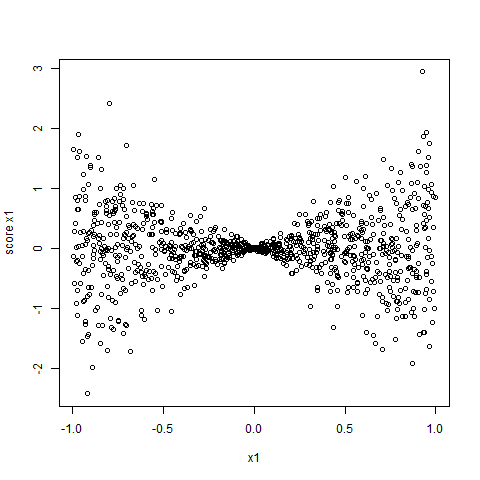
\includegraphics[width=1\textwidth]{Figures/Scores/correctly_specified_scores_x1_x1.png} 
    \end{minipage}\hfill
    \begin{minipage}{0.45\textwidth}
        \centering
        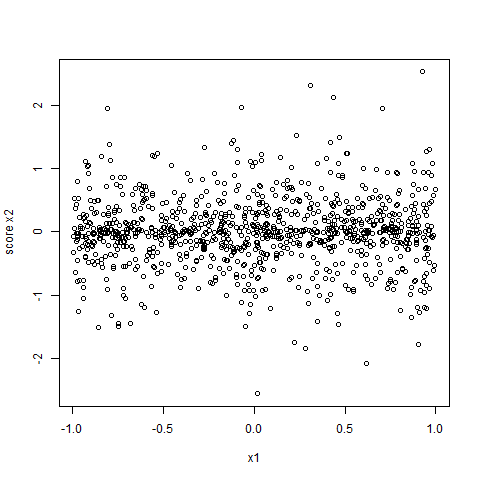
\includegraphics[width=1\textwidth]{Figures/Scores/correctly_specified_scores_x2_x1.png} 
    \end{minipage}
\end{figure}

\end{frame}

\begin{frame}{Scores}
If the data generating process $y = 1 + x_1 + x_2 + 3(I_{(x1<0)}) \cdot x_2 + eps$ includes an interaction term which is not specified in the model the scores ordered by $x_{1}$ are
\begin{figure}
    \centering
    \begin{minipage}{0.45\textwidth}
        \centering
        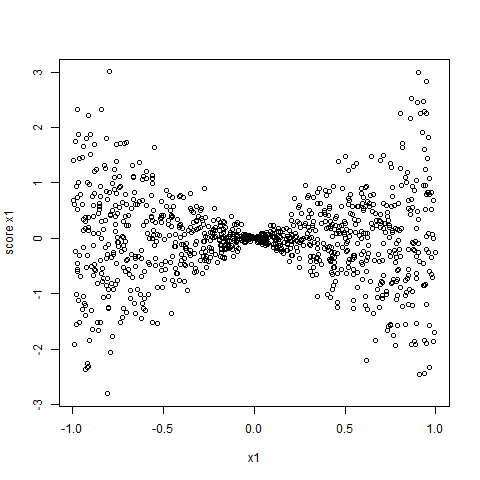
\includegraphics[width=1\textwidth]{Figures/Scores/misspecified_scores_x1_x1.png} 
    \end{minipage}\hfill
    \begin{minipage}{0.45\textwidth}
        \centering
        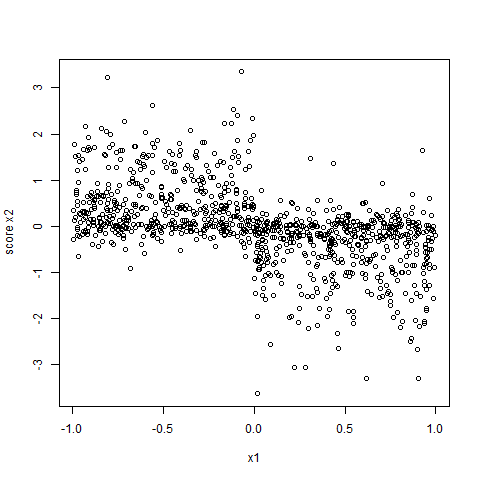
\includegraphics[width=1\textwidth]{Figures/Scores/misspecified_scores_x2_x1.png} 
    \end{minipage}
\end{figure}
    
\end{frame}


\begin{frame}{Scores}
The scores ordered by $x_{2}$ are
\begin{figure}
    \centering
    \begin{minipage}{0.45\textwidth}
        \centering
        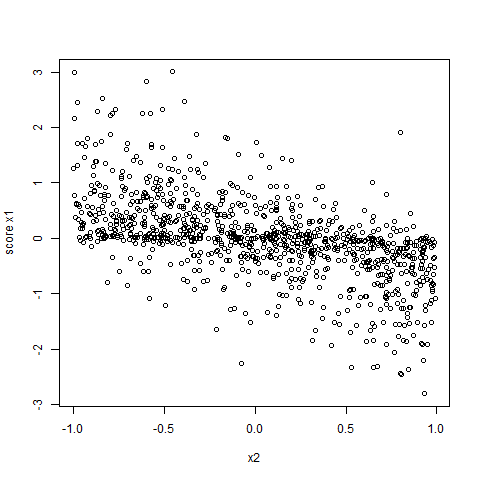
\includegraphics[width=1\textwidth]{Figures/Scores/misspecified_scores_x1_x2.png} 
    \end{minipage}\hfill
    \begin{minipage}{0.45\textwidth}
        \centering
        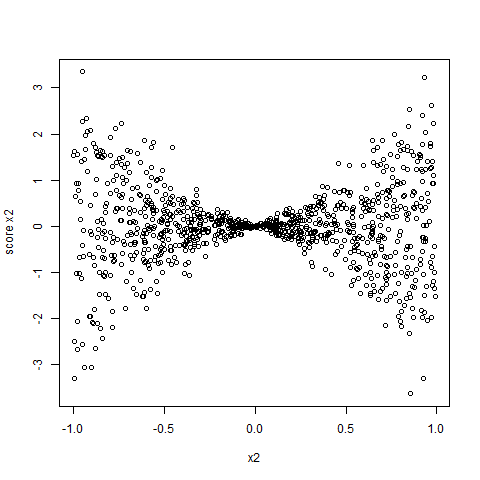
\includegraphics[width=1\textwidth]{Figures/Scores/misspecified_scores_x2_x2.png} 
    \end{minipage}
\end{figure}
    
\end{frame}


\begin{frame}{Step 2: Testing for Parameter Instability}
\textbf{Task}: Find out whether the parameters of the fitted model are stable over each particular ordering implied by the partitioning variables $Z_{j}$ 

\vspace{0.5cm}
\textbf{Idea}: check whether the scores $\hat{\psi_{i}}$ fluctuate randomly around their mean 0 or exhibit systematic deviations from 0 over $Z_{j}$
These deviations can be captured by the empirical fluctuation process
\begin{align}
    W_{j}(t) = \hat{J}^{-1/2}n^{-1/2}\sum_{i = 1}^{\lfloor nt \rfloor} \hat{\psi}_{\sigma(Z_{ij})} \hspace{0.5cm} (0 \leq t \leq 1), 
\end{align}

where $\hat{\psi}_{\sigma(Z_{ij})}$ are the scores ordered by $Z_{j}$ and $\hat{J}$ is an estimate of the covariance matrix $cov(\psi(Y, \hat(\theta)))$.

\end{frame}


\begin{frame}{Step 2: Testing for Parameter Instability}
\begin{itemize}
    \item Under the null hypothesis of parameter stability  $W_{j}(t)$ converges to a Brownian bridge $W^0$. \citep{Zeileis.2007}
    \item Various test statistics can be derived from $W_{j}(t)$ (e.g. supLM statistic for numeric variables).
The variable with the smallest p-value is then chosen as the best partitioning variable
\end{itemize}
    
\end{frame}

\begin{frame}{Applicability to our Task}
If the main effects of the potential partitioning variables are well fitted (e.g. through splines), their scores should fluctuate  around 0. Systematic deviations of the scores should then be due to interactions with other features. In my opinion, the test is therefore basically suitable for our question.

\vspace{0.5cm}

\textbf{Problems:}
\begin{itemize}
    \item Scores must be available, i.e. not usable for Lasso or MAE regression. For MAE regression robust regression could be an alternative.
    \item L2 penalization also seems to be problematic (\href{https://stackoverflow.com/questions/60767810/can-the-mob-function-in-partykit-build-model-trees-using-regularized-linear-mode/60775986##60775986}{stackoverflow})
\end{itemize}
\end{frame}


\subsection{CTree}
\begin{frame}{CTree: Conditional Inference Trees}
Conditional Inference Trees (CTree) work similar to MOB, but differ in the test for choosing the optimal partitioning variable

\vspace{0.5cm}

\textbf{Idea:} Test for each transformed split variable  $g(Z_{j})$ whether there is any association with the transformed response $h(Y)$.\citep{Schlosser.24.06.2019} 

\begin{itemize}
    \item a natural choice for $h()$ is the scorefunction $\psi(Y_{i}, \hat{\theta}) = \psi(Y_{i}, Z_{i}, \hat{\theta})$ (as used in MOB), but other transformations are also possible.
    \item Ctree uses a nonparametric test, i.e. in contrast to MOB no distribution assumption regarding $h(Y)$ has to be considered.
\end{itemize}


\end{frame}

\begin{frame}{Permutation Test}
Hypotheses: $H_0^j: D(Y|Z_{j}) = D(Y)$

\vspace{0.5cm}

Measure the association between $Y$ and $Z_{j}, j = 1,...,k$ by linear statistics of the form 
\begin{align}
    T_{j}(Y,Z) = vec\left(\sum_{i=1}^n g_{j}(Z_{ji})h(Y_{i})^T\right) \in \mathbb{R}^{p_{j}q}
\end{align}
\citep{Hothorn.2006}

Calculate the conditional expectation $\mu_{i}$ and covariance of $T_{j}$ under $H_{0}$ given all permutations of $S(\{Y,Z\})$ to standardize $T_{j}$ .

$$ \mu_{j} = \mathbb{E}\left(T_{j}({Y,Z})|S(({Y,Z)})\right) = vec\left(\left(\sum_{i=1}^n g_{j}(Z_{ji})\right)\frac{1}{n}\left(\sum_{i=1}^n h(Y_{i})\right)^T\right) $$

The standardized test statistic has than an asymptotic normal distribution.

\citep{Schlosser.24.06.2019}
\end{frame}


\begin{frame}{Applicability to our Task}
If the main effects of potential partitioning variable are well fitted, dependencies between scores and the partitioning variable should again be due to interactions with other features.

\vspace{0.5cm}

\textbf{Question}: Does the test detect dependencies reliably?

\vspace{0.5cm}

\textbf{Advantage}:
Association test is not limited to scores, i.e., unlike MOB, alternative transformations $h(Y)$ could be chosen for Lasso or MAE (e.g. Residuals).

However, the choice of a suitable transformation is difficult.


\end{frame}



\subsection{Comparsion}
\begin{frame}{Comparison of the methods based on examples}
 Simulation of 1000 observations  
\begin{align*}
     y = 1 + x_1 + x_2 + 3(I_{(x1<0)}) \cdot x_2 + eps
\end{align*}
with predictors $x_{1},x_{2}$ iid $U(-1,1)$ and $\epsilon \sim N(0,1)$

\vspace{0.5cm}
\textbf{Results}:
\begin{itemize}
    \item MOB and SLIM find the correct split at approximatly $x_1 = 0$
    \item CTree does not find the correct split and instead splits twice with respect to $x_2$ 
\end{itemize}
\end{frame}




\begin{frame}{Comparison of the methods based on examples}
\textbf{Simulation Data with two-way and three-way Interactions \citep{Hu.2020}}
Simulation of 10000 observations.
\begin{align*}
y = & 3x_{1} + x_{2}^3 - \pi^{x_{3}} + exp(-2x_{4}^2) + \frac{1}{2+|x_{5}|} + x_{6}log|x_{6}| \\
& + \sqrt{2|x_{7}|} + max(0,x_{7}) + x_{8}^4 + 2cos(\pi x_{8}) \\
& + 2(I_{x1>0})(I_{x2>0}) + 2(I_{x1>0})x_{4} + 4(x_{5}(I_{x5>0}))^{|x_{6}|} + |x_7 + x_8| + \epsilon
\end{align*}

with predictors $x_{1},...,x_{10}$ iid $U(-1,1)$ and $\epsilon \sim N(0,0.5^2)$.

\begin{itemize}
    \item Tune and train XGBoost model
    \item Use predictions as response for the surrogate trees
    \item Use SLIM, MOB and CTree to generate Model based trees 
\end{itemize}

\end{frame}



\begin{frame}{Comparison of the methods based on examples - Results}
\textbf{Bspline Transformations to all numeric features}
\begin{itemize}
    \item in all three methods $x_{1}$ is correctly chosen as the first partitioning variable 
    \item MOB and SLIM also find the same partitioning variables at level 2, CTree differs from here
\end{itemize}

\textbf{Polynomial Regression (degree 3)}
\begin{itemize}
    \item in all three methods $x_{8}$ is chosen as the first partitioning variable 
    \item the component $x_{8}^4$ cannot be well fitted with 3-degree polynomial. Therefore the split trys to fix this

\end{itemize}
    
\end{frame}

\begin{frame}{Comparison of the methods based on examples}
\textbf{Realworld example: Bike sharing \citep{Hu.2020}}

Data: hourly observations of bike rental counts, weather and time information
\begin{itemize}
    \item Tune and train XGBoost model with 11 predictors to predict hourly rental (log-) counts
    \item Use predictions as response for the surrogate trees
    \item Use SLIM, MOB and CTree to generate Model based trees (Linear Regression with bspline Transformations to all numeric features)
\end{itemize}

\vspace{0.5cm}
\textbf{Results}
\begin{itemize}
    \item SLIM and MOB choose the same variables for partitioning: First split on workingday yes/no. If yes, second split on temperature (Agrees with the result in the paper)
    \item CTree uses different variables for partitioning
\end{itemize}
\end{frame}


\section{Outlook}

\begin{frame}{Outlook}
\begin{itemize}
    \item full implementation of SLIM
    \item comparison of SLIM and MOB (possibly CTree)
    \item Combination of SLIM and MOB or Ctree, i.e.: Selection of the splitting variable via hypothesis testing. If scores are not available, check whether residuals can be used instead and whether the instability of the parameters is reflected in them (by means of efp or permutation test)
\end{itemize}
    
\end{frame}

    

\begin{frame}{Bibliography}
    \bibliography{bibliography}
    \bibliographystyle{dcu}

\end{frame}



\end{document}
